\documentclass{article}
\usepackage[final,main]{neurips_2025}  % NEURIPS style (camera-ready, main track)

\usepackage[utf8]{inputenc}
\usepackage[T1]{fontenc}
\usepackage[hidelinks]{hyperref}  % clickable links
\usepackage{booktabs}             % professional tables
\usepackage{graphicx}
\usepackage{amsmath,amssymb}
\usepackage{subcaption}
\usepackage{xspace}
\usepackage{enumitem}
\usepackage{multirow}
\usepackage{algorithm}
\usepackage[noend]{algpseudocode}

% Import command files
\input{commands/math}
\input{commands/general}
%%%%% PROJECT-SPECIFIC MACROS %%%%%
% Grounded ideation ablation paper
% Import with: %%%%% PROJECT-SPECIFIC MACROS %%%%%
% Grounded ideation ablation paper
% Import with: %%%%% PROJECT-SPECIFIC MACROS %%%%%
% Grounded ideation ablation paper
% Import with: \input{commands/macros}

\usepackage{xspace}

%%%%%%%%%%%%%%%%%%%%%%%%%%%%%%%%%%%%%%%%%%%%%%%%%%%%%%%%%%%%%%%%%
% REGIME / CONDITION NAMES
%%%%%%%%%%%%%%%%%%%%%%%%%%%%%%%%%%%%%%%%%%%%%%%%%%%%%%%%%%%%%%%%%

\newcommand{\Cungrounded}{\textsc{Ungrounded}\xspace}
\newcommand{\Cdeduction}{\textsc{Deduction}\xspace}
\newcommand{\Cinduction}{\textsc{Induction}\xspace}
\newcommand{\Cempirical}{\textsc{Empirical}\xspace}
\newcommand{\Cliterature}{\textsc{LitCompare}\xspace}
\newcommand{\Cproposal}{\textsc{Proposal}\xspace}

%%%%%%%%%%%%%%%%%%%%%%%%%%%%%%%%%%%%%%%%%%%%%%%%%%%%%%%%%%%%%%%%%
% DATASET NAMES
%%%%%%%%%%%%%%%%%%%%%%%%%%%%%%%%%%%%%%%%%%%%%%%%%%%%%%%%%%%%%%%%%

\newcommand{\headline}{\textsc{Headline}\xspace}
\newcommand{\deceptive}{\textsc{Deceptive}\xspace}
\newcommand{\dreaddit}{\textsc{Dreaddit}\xspace}

%%%%%%%%%%%%%%%%%%%%%%%%%%%%%%%%%%%%%%%%%%%%%%%%%%%%%%%%%%%%%%%%%
% MODEL AND METHOD NAMES
%%%%%%%%%%%%%%%%%%%%%%%%%%%%%%%%%%%%%%%%%%%%%%%%%%%%%%%%%%%%%%%%%

\newcommand{\gptmini}{\textsc{gpt-4.1-mini}\xspace}
\newcommand{\hypogenic}{\textsc{HypoGeniC}\xspace}
\newcommand{\scimon}{\textsc{SciMON}\xspace}
\newcommand{\hypobench}{\textsc{HypoBench}\xspace}

%%%%%%%%%%%%%%%%%%%%%%%%%%%%%%%%%%%%%%%%%%%%%%%%%%%%%%%%%%%%%%%%%
% ABBREVIATIONS
%%%%%%%%%%%%%%%%%%%%%%%%%%%%%%%%%%%%%%%%%%%%%%%%%%%%%%%%%%%%%%%%%

\newcommand{\ie}{i.e.,\xspace}
\newcommand{\eg}{e.g.,\xspace}
\newcommand{\IND}{\textsc{ind}\xspace}
\newcommand{\OOD}{\textsc{ood}\xspace}


\usepackage{xspace}

%%%%%%%%%%%%%%%%%%%%%%%%%%%%%%%%%%%%%%%%%%%%%%%%%%%%%%%%%%%%%%%%%
% REGIME / CONDITION NAMES
%%%%%%%%%%%%%%%%%%%%%%%%%%%%%%%%%%%%%%%%%%%%%%%%%%%%%%%%%%%%%%%%%

\newcommand{\Cungrounded}{\textsc{Ungrounded}\xspace}
\newcommand{\Cdeduction}{\textsc{Deduction}\xspace}
\newcommand{\Cinduction}{\textsc{Induction}\xspace}
\newcommand{\Cempirical}{\textsc{Empirical}\xspace}
\newcommand{\Cliterature}{\textsc{LitCompare}\xspace}
\newcommand{\Cproposal}{\textsc{Proposal}\xspace}

%%%%%%%%%%%%%%%%%%%%%%%%%%%%%%%%%%%%%%%%%%%%%%%%%%%%%%%%%%%%%%%%%
% DATASET NAMES
%%%%%%%%%%%%%%%%%%%%%%%%%%%%%%%%%%%%%%%%%%%%%%%%%%%%%%%%%%%%%%%%%

\newcommand{\headline}{\textsc{Headline}\xspace}
\newcommand{\deceptive}{\textsc{Deceptive}\xspace}
\newcommand{\dreaddit}{\textsc{Dreaddit}\xspace}

%%%%%%%%%%%%%%%%%%%%%%%%%%%%%%%%%%%%%%%%%%%%%%%%%%%%%%%%%%%%%%%%%
% MODEL AND METHOD NAMES
%%%%%%%%%%%%%%%%%%%%%%%%%%%%%%%%%%%%%%%%%%%%%%%%%%%%%%%%%%%%%%%%%

\newcommand{\gptmini}{\textsc{gpt-4.1-mini}\xspace}
\newcommand{\hypogenic}{\textsc{HypoGeniC}\xspace}
\newcommand{\scimon}{\textsc{SciMON}\xspace}
\newcommand{\hypobench}{\textsc{HypoBench}\xspace}

%%%%%%%%%%%%%%%%%%%%%%%%%%%%%%%%%%%%%%%%%%%%%%%%%%%%%%%%%%%%%%%%%
% ABBREVIATIONS
%%%%%%%%%%%%%%%%%%%%%%%%%%%%%%%%%%%%%%%%%%%%%%%%%%%%%%%%%%%%%%%%%

\newcommand{\ie}{i.e.,\xspace}
\newcommand{\eg}{e.g.,\xspace}
\newcommand{\IND}{\textsc{ind}\xspace}
\newcommand{\OOD}{\textsc{ood}\xspace}


\usepackage{xspace}

%%%%%%%%%%%%%%%%%%%%%%%%%%%%%%%%%%%%%%%%%%%%%%%%%%%%%%%%%%%%%%%%%
% REGIME / CONDITION NAMES
%%%%%%%%%%%%%%%%%%%%%%%%%%%%%%%%%%%%%%%%%%%%%%%%%%%%%%%%%%%%%%%%%

\newcommand{\Cungrounded}{\textsc{Ungrounded}\xspace}
\newcommand{\Cdeduction}{\textsc{Deduction}\xspace}
\newcommand{\Cinduction}{\textsc{Induction}\xspace}
\newcommand{\Cempirical}{\textsc{Empirical}\xspace}
\newcommand{\Cliterature}{\textsc{LitCompare}\xspace}
\newcommand{\Cproposal}{\textsc{Proposal}\xspace}

%%%%%%%%%%%%%%%%%%%%%%%%%%%%%%%%%%%%%%%%%%%%%%%%%%%%%%%%%%%%%%%%%
% DATASET NAMES
%%%%%%%%%%%%%%%%%%%%%%%%%%%%%%%%%%%%%%%%%%%%%%%%%%%%%%%%%%%%%%%%%

\newcommand{\headline}{\textsc{Headline}\xspace}
\newcommand{\deceptive}{\textsc{Deceptive}\xspace}
\newcommand{\dreaddit}{\textsc{Dreaddit}\xspace}

%%%%%%%%%%%%%%%%%%%%%%%%%%%%%%%%%%%%%%%%%%%%%%%%%%%%%%%%%%%%%%%%%
% MODEL AND METHOD NAMES
%%%%%%%%%%%%%%%%%%%%%%%%%%%%%%%%%%%%%%%%%%%%%%%%%%%%%%%%%%%%%%%%%

\newcommand{\gptmini}{\textsc{gpt-4.1-mini}\xspace}
\newcommand{\hypogenic}{\textsc{HypoGeniC}\xspace}
\newcommand{\scimon}{\textsc{SciMON}\xspace}
\newcommand{\hypobench}{\textsc{HypoBench}\xspace}

%%%%%%%%%%%%%%%%%%%%%%%%%%%%%%%%%%%%%%%%%%%%%%%%%%%%%%%%%%%%%%%%%
% ABBREVIATIONS
%%%%%%%%%%%%%%%%%%%%%%%%%%%%%%%%%%%%%%%%%%%%%%%%%%%%%%%%%%%%%%%%%

\newcommand{\ie}{i.e.,\xspace}
\newcommand{\eg}{e.g.,\xspace}
\newcommand{\IND}{\textsc{ind}\xspace}
\newcommand{\OOD}{\textsc{ood}\xspace}


\bibliographystyle{plainnat}

\title{When Does Grounding Help LLM Ideation?\\ A Single-Protocol Ablation of Six Grounding Mechanisms}

\author{Chenhao Tan and NeuriCo}

\begin{document}
\maketitle

\begin{abstract}
A popular prescription for automated scientific ideation is to \emph{ground} the
process---in deduction, induction, small experiments, literature comparison, or
proposal writing---rather than prompting a language model abstractly. Yet every
prior method grounds in only one way and compares against a (typically weak)
ungrounded baseline, so it remains unknown which grounding \emph{mechanism}
actually helps when all else is held fixed. We present the first single-protocol,
head-to-head ablation of six ideation regimes (one ungrounded control plus five
grounding mechanisms). Holding the model (\gptmini), task suite, generation
budget, and evaluation procedure fixed, each regime produces a bank of $15$ task
hypotheses, and each bank is scored by an objective downstream-utility metric: how
accurately an LLM applying the bank predicts held-out labels, both in-distribution
(\IND) and out-of-distribution (\OOD), across three classification tasks and three
seeds ($54$ banks, $\approx 11.9$k API calls). We find that grounding does
\emph{not} uniformly help: pooled across regimes, grounded banks are statistically
indistinguishable from---and slightly below---the ungrounded control. But the
mechanism matters decisively. Grounding in \emph{empirical feedback}
(test-and-revise) is the only regime that significantly improves \IND{} accuracy
($+4.4$ points, Cohen's $d=1.09$, $p=0.02$), at roughly $80\times$ the token cost;
proposal writing significantly \emph{hurts} ($-5.7$ points, $p=0.008$) and
collapses idea diversity; and data grounding can \emph{overfit}, trading \OOD{}
robustness for \IND{} fit. Novelty and diversity do not track usefulness within a
task. For today's strong LLMs, ``ground your ideation'' is too coarse: only
empirical grounding reliably adds value, and ungrounded prompting is a
surprisingly hard baseline to beat.

\end{abstract}

\section{Introduction}
\label{sec:intro}

Can large language models (LLMs) generate \emph{good} scientific ideas? Skepticism
is widespread: model-generated hypotheses tend to be either incremental or
implausibly radical, and ``novelty'' itself resists definition~\citep{si2024llm}.
A recurring answer in recent work is to \emph{ground} ideation rather than prompt
for ideas abstractly. SciMON grounds in retrieved literature~\citep{wang2023scimon};
HypoGeniC grounds in labeled data~\citep{zhou2024hypogenic}; ResearchAgent grounds
in structured proposals~\citep{baek2024researchagent}; and SGA grounds in simulation
feedback~\citep{ma2024sga}. Each reports that its grounded method beats an
ungrounded prompt.

\para{Why this matters.} If we can say \emph{which kinds of grounding} turn raw LLM
ideation into useful ideas---and at what cost---we give practitioners a concrete
recipe and move the field past single-number ``novelty'' leaderboards toward
grounded usefulness. This is increasingly urgent because the ungrounded baseline is
a moving target: the 2023-era finding that grounding helps was measured against much
weaker models, and a strong modern LLM may already encode much of what grounding was
meant to supply.

\para{The gap.} Every prior method grounds in \emph{one} way and compares to an
ungrounded prompt. Nobody has held task, model, generation budget, and evaluation
metric fixed and ablated the grounding \emph{mechanisms} against each other. So we
cannot say whether literature comparison, induction, empirical feedback, deduction,
or proposal writing is responsible for the reported gains---or whether, with a strong
2025 model, any of them still helps. We also heed the field's central caveat, that
novelty is over-trusted and can flip once ideas are executed~\citep{si2024llm}, by
scoring \emph{grounded usefulness} rather than a bare novelty score.

\para{Our approach.} We build the first single-protocol, head-to-head ablation of
six ideation regimes: one ungrounded control (C0) and five grounding mechanisms
(deduction, induction, empirical small-experiments/outcome-imagination, literature
comparison, and proposal writing). We operationalize an ``idea'' as a \emph{task
hypothesis}---an explicit decision rule explaining a binary classification
phenomenon---and ``better'' as how accurately an LLM applying a bank of $15$ such
hypotheses predicts held-out labels, in-distribution (\IND) and out-of-distribution
(\OOD). Holding the model (\gptmini), bank size, and an identical evaluator fixed,
the \emph{only} variable is how the ideas were grounded. We run all six regimes on
three \hypogenic{} tasks across three seeds ($54$ banks, $\approx 11.9$k API calls,
$\approx\$3$), and complement accuracy with diversity, a novelty--usefulness
analysis, and a cost/benefit accounting.

\para{What we find.} Grounding does not uniformly help. Pooled across regimes,
grounded banks are statistically indistinguishable from---and slightly below---the
ungrounded control (\IND{} $-1.2$ pts, \OOD{} $-2.5$ pts, both n.s.). But the
mechanism matters decisively: empirical small-experiment grounding is the only
regime that significantly improves \IND{} accuracy ($+4.4$ pts, Cohen's $d=1.09$,
$p=0.02$), while proposal writing significantly \emph{hurts} ($-5.7$ pts, $d=-1.56$,
$p=0.008$) and collapses diversity. Data grounding can \emph{overfit}: on deceptive
reviews the ungrounded model transfers near-perfectly \OOD{} ($0.97$) using general
priors, whereas data-grounded rules latch onto dataset-specific surface cues and drop
to $0.78$--$0.82$ \OOD. Empirical grounding's gains cost roughly $80\times$ the
generation tokens of the control.

\para{Contributions.}
\begin{itemize}[leftmargin=*,itemsep=0pt,topsep=2pt]
    \item We conduct the first single-protocol, head-to-head ablation of six LLM
    ideation regimes, holding model, task suite, generation budget, and evaluation
    fixed and scoring each by objective downstream utility (\IND{} and \OOD{}
    accuracy).
    \item We show that grounding does not uniformly help a strong LLM, and isolate
    the one mechanism that does: grounding in empirical feedback (test-and-revise)
    is the only regime that significantly improves in-distribution usefulness.
    \item We surface two cautions the field under-reports: pure elaboration
    (proposal writing) actively degrades idea quality and diversity, and data
    grounding can trade out-of-distribution robustness for in-distribution fit.
    \item We complement accuracy with diversity, a novelty--usefulness analysis (a
    task-difficulty confound that vanishes within task), and a cost/benefit
    accounting, and release all banks, predictions, and statistics for reproducibility.
\end{itemize}

The rest of the paper reviews related work (\secref{sec:related}), details the
protocol and six regimes (\secref{sec:method}), presents results
(\secref{sec:results}), and discusses implications and limitations
(\secref{sec:discussion}).

\section{Related Work}
\label{sec:related}

\para{Literature-grounded ideation.} A large body of work grounds idea generation
in retrieved prior art. \scimon{} retrieves inspirations and runs an iterative
``novelty-boosting'' loop that forces each idea to differ from its $k$ nearest
neighbors, raising human-judged novelty for $46$--$58\%$ of
ideas~\citep{wang2023scimon}. ResearchAgent traverses citation graphs and an
entity knowledge store~\citep{baek2024researchagent}; Chain-of-Ideas induces the
developmental trend of a field before proposing~\citep{li2024coi}; Nova plans and
retrieves each round to keep ideas novel~\citep{hu2024nova}; and MOOSE-Chem composes
hypotheses from background plus deliberately non-neighboring
inspirations~\citep{yang2024moosechem}. We instantiate this family as our literature-
comparison regime, but---to keep the ablation leakage-controlled and single-model---we
differentiate against the model's own accumulating idea pool rather than an external
corpus. Unlike these systems, our goal is not to build a better literature-grounded
generator but to place literature comparison \emph{on the same footing} as other
grounding mechanisms.

\para{Data-driven and empirical grounding.} \hypogenic{} induces explanatory
hypotheses from labeled examples and refines them with a bandit-style
reward tied to predictive accuracy, beating few-shot prompting by $3.3$--$31.7\%$ and
even fine-tuned oracles~\citep{zhou2024hypogenic}. Literature Meets Data shows
literature and data are complementary, improving \OOD{} accuracy by
$8.97\%$ over few-shot~\citep{liu2024literature}. SGA closes the loop with a
differentiable simulator, where removing the simulation grounding collapses
performance by orders of magnitude~\citep{ma2024sga}. \hypobench{} benchmarks these
methods at scale and finds data-driven and literature+data methods dominate
inference-only and zero-shot-generation baselines, especially
\OOD~\citep{liu2025hypobench}. Our induction and empirical regimes are direct,
minimal instantiations of this line; our contribution is to measure them against the
\emph{same} ungrounded control and each other, and to report when data grounding
\emph{overfits} rather than transfers.

\para{Proposal-writing and structured ideation.} Several systems ground ideation by
writing full structured proposals (problem $\rightarrow$ method $\rightarrow$
experiments) that are critiqued and revised~\citep{baek2024researchagent,si2024llm}.
\citet{si2024llm} find LLM proposals are judged more novel than expert humans but
slightly less feasible. We include proposal writing as a regime and find that, when
distilled into decision rules, it can \emph{reduce} usefulness and diversity---a
concrete case of an idea looking thorough while being less useful.

\para{Evaluating ideas.} Because ``is this novel?'' prompts are unreliable, recent
work grounds the \emph{judgment} in retrieved literature: RAG-Novelty and
literature-grounded assessment beat ungrounded LLM-as-judge
prompting~\citep{lin2024schnovel,shahid2025litnovelty}, and idea-level benchmarks
catalog the trade-offs~\citep{guo2024ideabench,liu2025researchbench}. The consistent
caveat---\emph{novelty $\neq$ value}, sharpened by the ideation--execution flip of
\citet{si2024llm}---motivates our choice to score grounded usefulness (downstream
\IND/\OOD{} accuracy) rather than a bare novelty score, and to test the
novelty--usefulness relationship directly.

\para{Our position.} Every method above grounds in a single way and beats an
ungrounded prompt measured with a weaker model. We hold task, model, generation
budget, and evaluation fixed and ablate the grounding \emph{mechanisms} against one
another under one protocol. To our knowledge this head-to-head comparison does not
exist, and it yields a partly negative, mechanism-specific picture that the
single-grounding literature could not surface.

\section{Methodology}
\label{sec:method}

\para{Operationalizing the question.} We make ``idea quality'' objective and
leakage-controlled. An \newterm{idea} is a \emph{task hypothesis}: an explicit,
general decision rule explaining a binary classification phenomenon (\eg ``stressed
posts use more first-person pronouns and absolutist words''). ``\newterm{Better}''
is \emph{grounded usefulness}: when an LLM applies a full bank of $K=15$ hypotheses
to a new instance, how often it predicts the correct label. This reuses the
field-standard \hypogenic{} utility metric~\citep{zhou2024hypogenic} and lets us
compare grounding mechanisms apples-to-apples.

\subsection{Six ideation regimes}
\label{sec:regimes}

The independent variable is the ideation regime, with six levels: one ungrounded
control and five grounding mechanisms drawn directly from the strategies named in the
literature (\secref{sec:related}). \tabref{tab:regimes} summarizes them. Held fixed
across all regimes: the generator \gptmini{} ($T{=}0.7$), the bank size $K{=}15$, and
the identical evaluation procedure below. The only thing that varies is \emph{how the
ideas were grounded}. To avoid leakage, the dataset's expert \texttt{known\_hypotheses}
are \emph{never} shown during generation; the literature-comparison regime
differentiates against the model's own accumulating pool, not the expert set.

\begin{table}[t]
\centering
\caption{The six ideation regimes: one ungrounded control plus five grounding
mechanisms. Each generates a bank of $K{=}15$ task hypotheses under \gptmini.
Generation tokens per bank (rightmost) span nearly two orders of magnitude.}
\label{tab:regimes}
\resizebox{\textwidth}{!}{%
\begin{tabular}{@{}llp{3.0cm}p{5.6cm}r@{}}
\toprule
\textbf{ID} & \textbf{Regime} & \textbf{Grounding} & \textbf{What it sees / does} & \textbf{Tok/bank} \\
\midrule
C0 & \Cungrounded{} (control) & none & task description only $\rightarrow$ ``propose $15$ novel hypotheses'' & $460$ \\
C1 & \Cdeduction{}   & reasoning  & decompose causal mechanisms from first principles $\rightarrow$ derive rules & $918$ \\
C2 & \Cinduction{}   & data       & $20$ labeled examples $\rightarrow$ induce explanatory rules & $2{,}897$ \\
C3 & \Cempirical{}   & empirical feedback & induce, then \emph{test} the bank on fresh examples, observe errors, \emph{revise} ($2$ rounds) & $36{,}935$ \\
C4 & \Cliterature{}  & comparison & generate in rounds, each forced to differ from the prior pool (\scimon-style) & $1{,}150$ \\
C5 & \Cproposal{}    & elaboration & write a structured proposal $\rightarrow$ distill into rules & $1{,}588$ \\
\bottomrule
\end{tabular}}
\end{table}

\subsection{Shared evaluator}
\label{sec:eval}

For every bank, a separate evaluator LLM (\gptmini, $T{=}0$) is shown the $15$
hypotheses plus one instance and must apply them to answer ``A'' or ``B''. The option
order is deterministically swapped per item to neutralize position bias. Unparseable
answers count as wrong (we track an abstain rate, which was $0.0\%$ everywhere). Each
bank is scored on $100$ \IND{}-test and $100$ \OOD{} items. Because the evaluator
prompt and items are identical across regimes, differences in accuracy reflect
differences in the \emph{hypotheses}, not the inference procedure.

\subsection{Datasets}
\label{sec:data}

We use three \hypogenic{} \emph{real} tasks, all balanced $50/50$: \headline{} (which
of two headlines gets more clicks), \deceptive{} (fake vs.\ genuine hotel review), and
\dreaddit{} (stress vs.\ no-stress Reddit post). Each ships a task description and a set
of expert \texttt{known\_hypotheses}, which we hold out as a novelty anchor and an
approximate topline reference (never shown during generation). \deceptive{} and
\dreaddit{} provide an \OOD{} split from a different source/domain; for \headline{} we
use a disjoint held-out split.

\subsection{Baselines and statistics}
\label{sec:stats}

The ungrounded control C0 is the key reference; chance/majority is $0.50$ (balanced
tasks), and the expert known-hypotheses bank is an approximate topline. With $3$ seeds
$\times\, 3$ tasks we have $9$ paired cells per regime. Our primary test compares each
grounded regime against C0, paired across cells, using the Wilcoxon signed-rank test
and a paired $t$-test, reporting Cohen's $d$ effect size and applying a Bonferroni
correction over the $5$ grounded-vs-control comparisons. We compute bootstrap $95\%$
confidence intervals ($10$k resamples) over the pooled test items ($n{=}900$ per
regime per split). We set $\alpha=0.05$.

\subsection{Reproducibility and cost}
\label{sec:repro}

Seeds are fixed and every API call is disk-cached for idempotent reruns; banks,
per-item predictions, and statistics are all saved. The full study ($3$ tasks
$\times\, 6$ regimes $\times\, 3$ seeds, $100$ \IND{} $+\, 100$ \OOD{} eval items)
used $7.19$M input and $44.8$k output tokens across $11{,}931$ calls ($\approx\$3$),
with a wall-clock of $\approx 14$ minutes at $32$-way concurrency. No GPU is required;
the pipeline is API-only.

\section{Results}
\label{sec:results}

We organize results around four questions: Does grounding help overall
(\secref{sec:res-aggregate})? Which mechanism helps, and is it significant
(\secref{sec:res-sig})? How does the answer vary by task
(\secref{sec:res-pertask})? And do novelty, diversity, and cost track usefulness
(\secref{sec:res-novelty})?

\subsection{Grounding does not uniformly help}
\label{sec:res-aggregate}

\tabref{tab:aggregate} reports mean accuracy per regime, averaged over $3$ tasks
$\times\, 3$ seeds. The empirical regime (C3) has the best \IND{} accuracy
($0.676$), and the ungrounded control (C0) has the best \OOD{} accuracy ($0.760$).
Pooling the five grounded regimes against C0 (our H1 test), grounding is
statistically indistinguishable from---and slightly below---the control: \IND{}
$0.619$ vs.\ $0.631$ ($d{=}-0.32$, $p{=}0.37$) and \OOD{} $0.735$ vs.\ $0.760$
($d{=}-0.41$, $p{=}0.25$). The blanket claim ``grounding makes a strong LLM's ideas
better'' is \emph{not} supported.

\begin{table}[t]
\centering
\caption{Aggregate accuracy by regime (mean over $3$ tasks $\times\, 3$ seeds).
\textbf{Best per column in bold.} Grounding does not uniformly beat the ungrounded
control C0: C3 (empirical) is best \IND, but C0 is best \OOD. Diversity is mean
pairwise cosine distance within a bank; novelty distance is mean cosine distance to
the held-out expert hypotheses; generation tokens per bank span $\sim\!80\times$.}
\label{tab:aggregate}
\resizebox{\textwidth}{!}{%
\begin{tabular}{@{}lcccccccr@{}}
\toprule
\textbf{Regime} & \textbf{\IND{} acc} & \textbf{\IND{} sd} & \textbf{\OOD{} acc} & \textbf{\OOD{} sd} & \textbf{Diversity} & \textbf{Novelty} & \textbf{Gen tok/bank} \\
\midrule
C0 \Cungrounded{} (control) & $0.631$ & $.079$ & $\mathbf{0.760}$ & $.183$ & $0.417$ & $0.399$ & $\mathbf{460}$ \\
C1 \Cdeduction{}           & $0.608$ & $.071$ & $0.766$ & $.166$ & $0.367$ & $0.399$ & $918$ \\
C2 \Cinduction{}           & $0.637$ & $.053$ & $0.719$ & $.113$ & $0.409$ & $0.431$ & $2{,}897$ \\
C3 \Cempirical{}           & $\mathbf{0.676}$ & $.095$ & $0.739$ & $.117$ & $0.392$ & $0.430$ & $36{,}935$ \\
C4 \Cliterature{}          & $0.601$ & $.032$ & $0.721$ & $.175$ & $0.396$ & $0.415$ & $1{,}150$ \\
C5 \Cproposal{}            & $0.574$ & $.070$ & $0.729$ & $.183$ & $0.308$ & $0.415$ & $1{,}588$ \\
\bottomrule
\end{tabular}}
\end{table}

\begin{figure}[t]
\centering
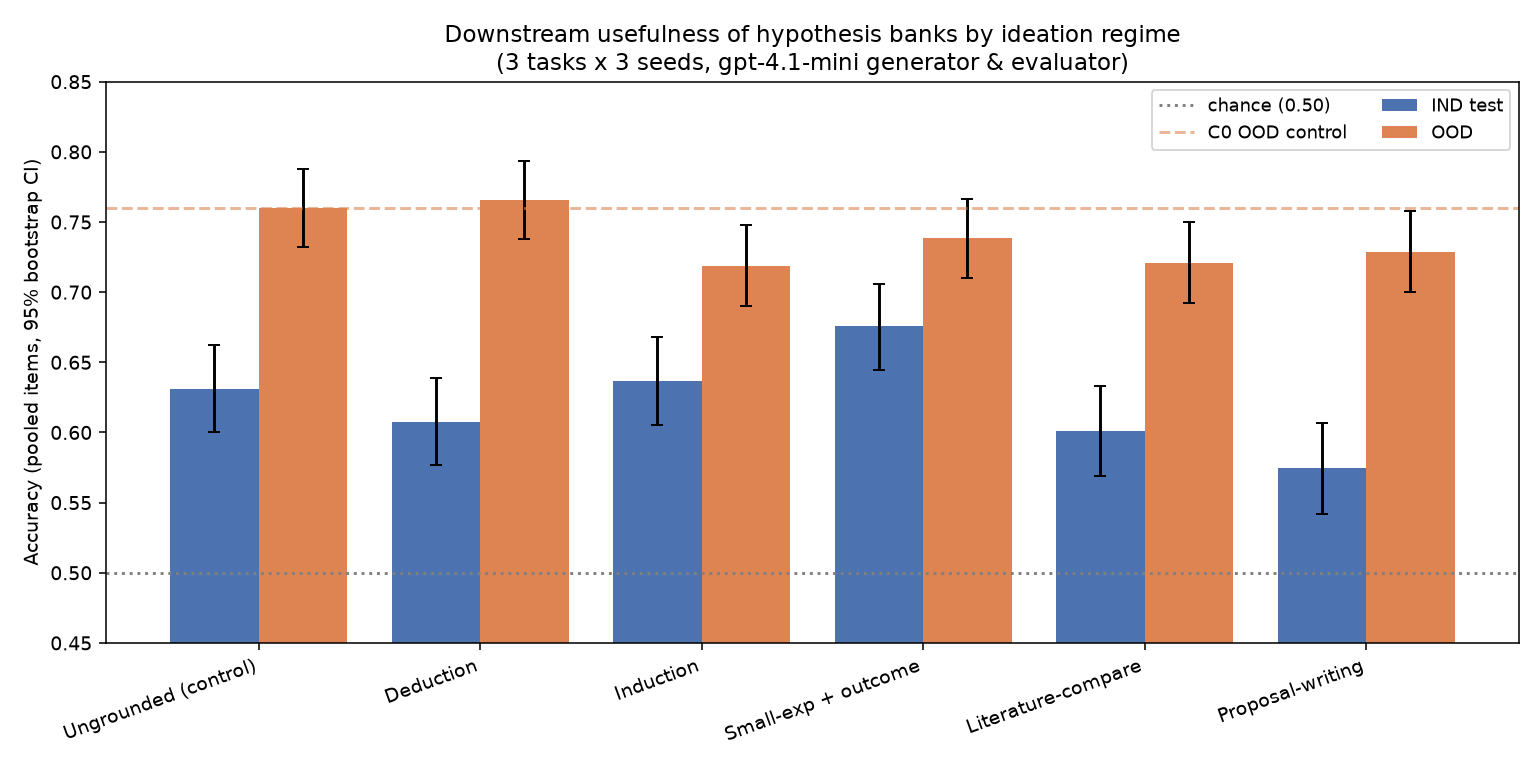
\includegraphics[width=0.95\linewidth]{figures/fig1_accuracy_by_regime.png}
\caption{In-distribution (\IND) and out-of-distribution (\OOD) accuracy by regime,
with bootstrap $95\%$ confidence intervals. The empirical regime (C3) leads
\IND; the ungrounded control (C0) leads \OOD. The chance line is at $0.50$. Mean
differences between most grounded regimes and the control are small relative to the
confidence intervals.}
\label{fig:accuracy}
\end{figure}

\subsection{The mechanism matters: empirical grounding helps, proposal writing hurts}
\label{sec:res-sig}

\tabref{tab:significance} gives the paired comparison of each grounded regime against
the control. Two regimes move the needle, in opposite directions. \Cempirical{} (C3)
is the only regime that \emph{significantly improves} \IND{} accuracy ($+0.044$,
$d{=}1.09$, Wilcoxon $p{=}0.020$); it is the one mechanism that changes its ideas in
response to evidence---it tests the bank, sees concrete mistakes, and revises.
\Cproposal{} (C5) \emph{significantly hurts} \IND{} accuracy ($-0.057$, $d{=}-1.56$,
$p{=}0.008$), surviving the Bonferroni correction, and it has by far the lowest
diversity ($0.308$ in \tabref{tab:aggregate}). The remaining regimes (deduction,
induction, literature comparison) are within noise of the control. No grounded regime
significantly beats the control \OOD. This supports H2 only partially---empirical
grounding leads on \IND, but the full predicted ordering does not hold---and refutes
H3: the grounding advantage is \emph{not} larger \OOD, and is often reversed
(\figref{fig:advantage}).

\begin{table}[t]
\centering
\caption{Paired significance of each grounded regime vs.\ the ungrounded control C0
($9$ paired task$\times$seed cells; Bonferroni $m{=}5$). \textbf{Bold} marks
significant effects ($p<0.05$). Empirical grounding (C3) is the only regime that
significantly improves \IND{} accuracy; proposal writing (C5) significantly hurts and
survives Bonferroni correction. No grounded regime significantly beats C0 \OOD.}
\label{tab:significance}
\resizebox{0.85\textwidth}{!}{%
\begin{tabular}{@{}llcccc@{}}
\toprule
\textbf{Split} & \textbf{Regime} & \textbf{Gain vs.\ C0} & \textbf{Cohen's $d$} & \textbf{Wilcoxon $p$} & \textbf{$t$ $p$ (Bonf.)} \\
\midrule
\IND{} & C1 \Cdeduction{}   & $-0.023$ & $-0.51$ & $0.195$ & $0.826$ \\
\IND{} & C2 \Cinduction{}   & $+0.006$ & $+0.11$ & $0.785$ & $1.000$ \\
\IND{} & \textbf{C3 \Cempirical{}} & $\mathbf{+0.044}$ & $\mathbf{+1.09}$ & $\mathbf{0.020}$ & $0.058$ \\
\IND{} & C4 \Cliterature{}  & $-0.030$ & $-0.46$ & $0.195$ & $1.000$ \\
\IND{} & \textbf{C5 \Cproposal{}} & $\mathbf{-0.057}$ & $\mathbf{-1.56}$ & $\mathbf{0.008}$ & $\mathbf{0.008}$ \\
\midrule
\OOD{} & C1 \Cdeduction{}   & $+0.006$ & $+0.14$ & $0.719$ & $1.000$ \\
\OOD{} & C2 \Cinduction{}   & $-0.041$ & $-0.29$ & $0.652$ & $1.000$ \\
\OOD{} & C3 \Cempirical{}   & $-0.021$ & $-0.19$ & $0.742$ & $1.000$ \\
\OOD{} & C4 \Cliterature{}  & $-0.039$ & $-0.54$ & $0.102$ & $0.715$ \\
\OOD{} & C5 \Cproposal{}    & $-0.031$ & $-0.47$ & $0.234$ & $0.988$ \\
\bottomrule
\end{tabular}}
\end{table}

\begin{figure}[t]
\centering
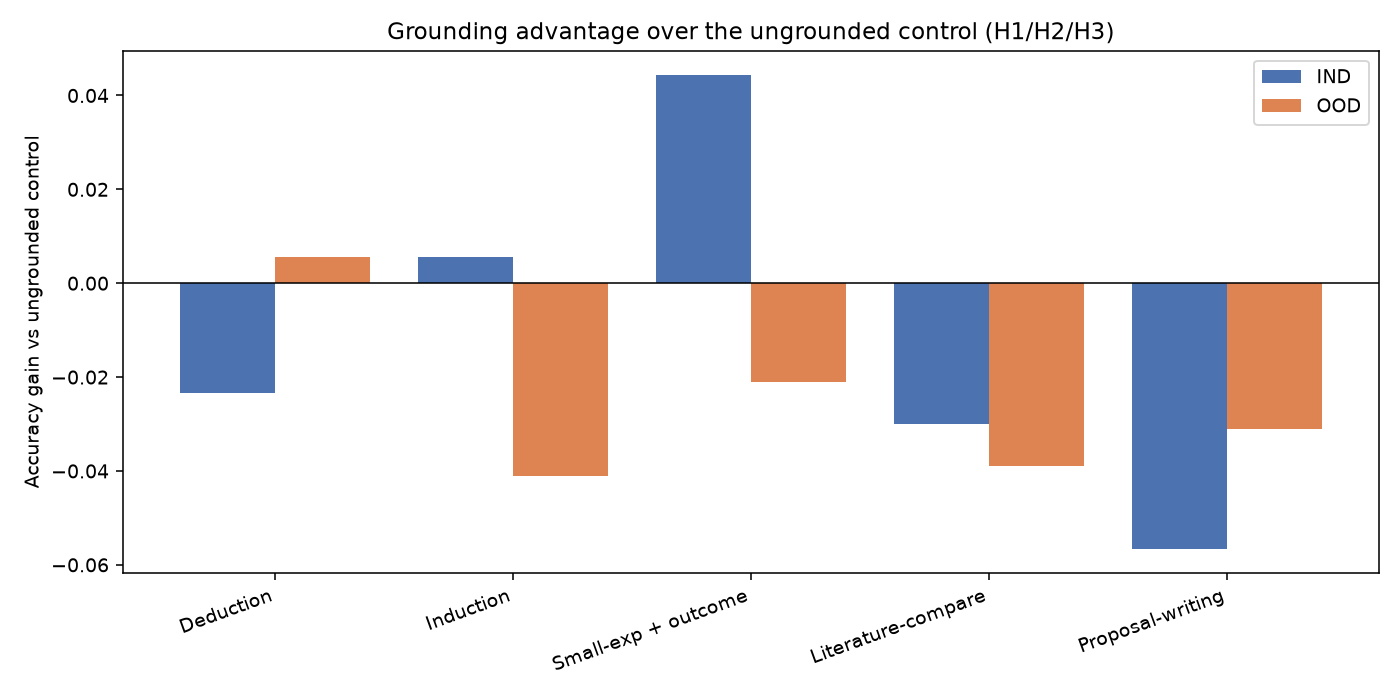
\includegraphics[width=0.7\linewidth]{figures/fig2_grounding_advantage.png}
\caption{Grounding advantage (regime accuracy minus control C0) on \IND{} and \OOD.
Only empirical grounding (C3) shows a clear positive \IND{} advantage; proposal
writing (C5) shows a clear negative one. Contrary to H3, advantages are not larger
\OOD---the \OOD{} bars are mostly negative.}
\label{fig:advantage}
\end{figure}

\subsection{Three tasks, three stories: heterogeneity and overfitting}
\label{sec:res-pertask}

The aggregate masks sharp per-task heterogeneity (\tabref{tab:pertask},
\figref{fig:heatmap}). On \dreaddit, empirical grounding (C3) wins clearly on
\emph{both} \IND{} ($0.78$ vs.\ $0.72$) and \OOD{} ($0.81$ vs.\ $0.75$)---here
grounding genuinely helps. On \deceptive, the ungrounded model transfers
near-perfectly \OOD{} ($0.97$) using general priors, while data grounding (C2/C3)
\emph{raises} \IND{} but \emph{crashes} \OOD{} to $0.78$--$0.82$: the learned rules
encode dataset-specific surface cues (\eg spatial/Chicago-hotel vocabulary) that do
not transfer, whereas the ungrounded prior captures general ``fake review'' structure
that does. This is the paper's most important nuance: \emph{data grounding can overfit},
trading \OOD{} robustness for \IND{} fit---a caution prior work, which emphasizes data
grounding's \OOD{} \emph{wins}, under-reports. On \headline, all regimes hover near
chance ($0.50$--$0.61$), including the expert hypotheses ($0.56/0.58$); there is little
extractable signal, so the task contributes mostly noise to the aggregate.

\begin{table}[t]
\centering
\caption{Per-task accuracy (\IND{} / \OOD, mean over seeds) for selected regimes.
\textbf{Bold} marks the best \IND/\OOD{} on a task among the shown regimes. Three
distinct stories: grounding helps on \dreaddit, overfits on \deceptive{} (ungrounded
\OOD{} $0.97$ vs.\ grounded $\le 0.82$), and finds no signal on \headline.}
\label{tab:pertask}
\resizebox{0.8\textwidth}{!}{%
\begin{tabular}{@{}lccc@{}}
\toprule
\textbf{Regime} & \textbf{\headline} & \textbf{\deceptive} & \textbf{\dreaddit} \\
\midrule
C0 \Cungrounded{} & $0.55 / 0.56$ & $0.62 / \mathbf{0.97}$ & $0.72 / 0.75$ \\
C2 \Cinduction{}  & $0.58 / 0.61$ & $0.65 / 0.78$ & $0.68 / 0.77$ \\
C3 \Cempirical{}  & $0.56 / 0.59$ & $\mathbf{0.69} / 0.82$ & $\mathbf{0.78} / \mathbf{0.81}$ \\
C5 \Cproposal{}   & $0.50 / 0.57$ & $0.58 / 0.97$ & $0.64 / 0.65$ \\
\bottomrule
\end{tabular}}
\end{table}

\begin{figure}[t]
\centering
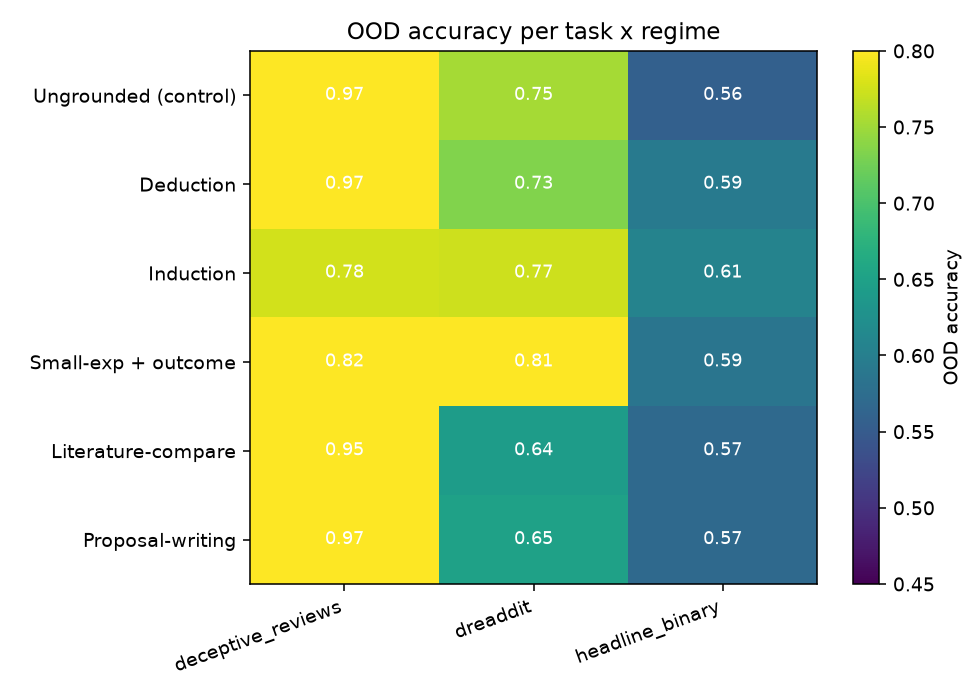
\includegraphics[width=0.95\linewidth]{figures/fig5_per_task_heatmap.png}
\caption{Per-task accuracy grid across all six regimes (\IND{} and \OOD).
The heterogeneity is stark: \dreaddit{} rewards grounding, \deceptive{} shows the
ungrounded control's near-perfect \OOD{} transfer collapsing under data grounding,
and \headline{} sits near chance throughout.}
\label{fig:heatmap}
\end{figure}

\subsection{Cost, novelty, and diversity do not buy usefulness}
\label{sec:res-novelty}

\para{Cost/benefit.} C3's \IND{} gain is expensive: it costs $\sim\!80\times$ the
generation tokens of the control ($36.9$k vs.\ $0.46$k tokens/bank), driven by its
test-and-revise loop (\figref{fig:cost}). The cheaper grounded regimes (C1, C4, C5 at
$0.9$k--$1.6$k tokens) do \emph{not} beat the control. Grounding's one reliable win
comes only at the top of the cost curve.

\para{Novelty $\neq$ usefulness.} Across the $18$ task$\times$regime cells,
Spearman$(\text{novelty},\,\OOD)=+0.835$ ($p<0.001$)---but this is a task-difficulty
confound (a Simpson's paradox): easy, high-accuracy tasks also have ideas farther from
their expert anchors. \emph{Within} a task the relationship vanishes (mean
$\rho\approx-0.10$; \deceptive{} $\rho=-0.75$), and diversity$\to$usefulness is weak
within task (mean $\rho\approx+0.33$, n.s.). Novelty and diversity are therefore not
reliable proxies for usefulness (\figref{fig:novelty}), consistent with the
literature's caveat and confirming H4 once the task confound is removed.

\begin{figure}[t]
\centering
\begin{subfigure}[b]{0.48\textwidth}
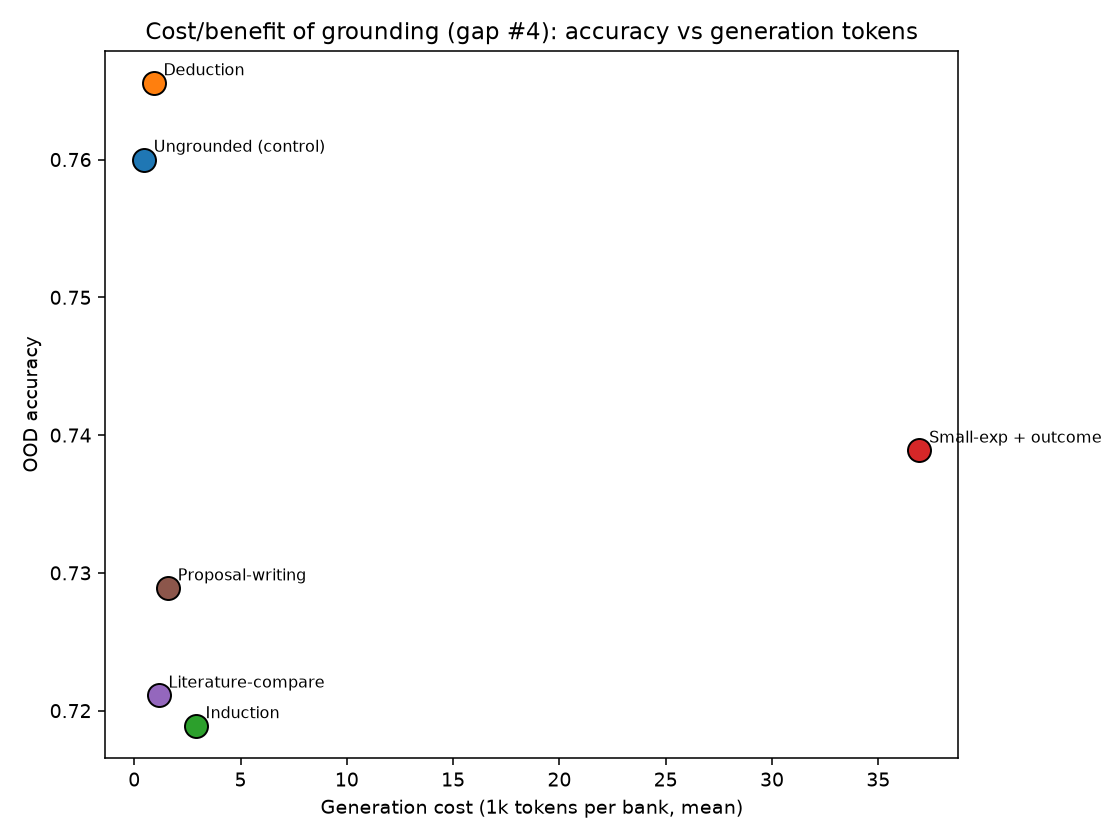
\includegraphics[width=\textwidth]{figures/fig4_cost_benefit.png}
\caption{Cost vs.\ benefit}
\label{fig:cost}
\end{subfigure}
\hfill
\begin{subfigure}[b]{0.48\textwidth}
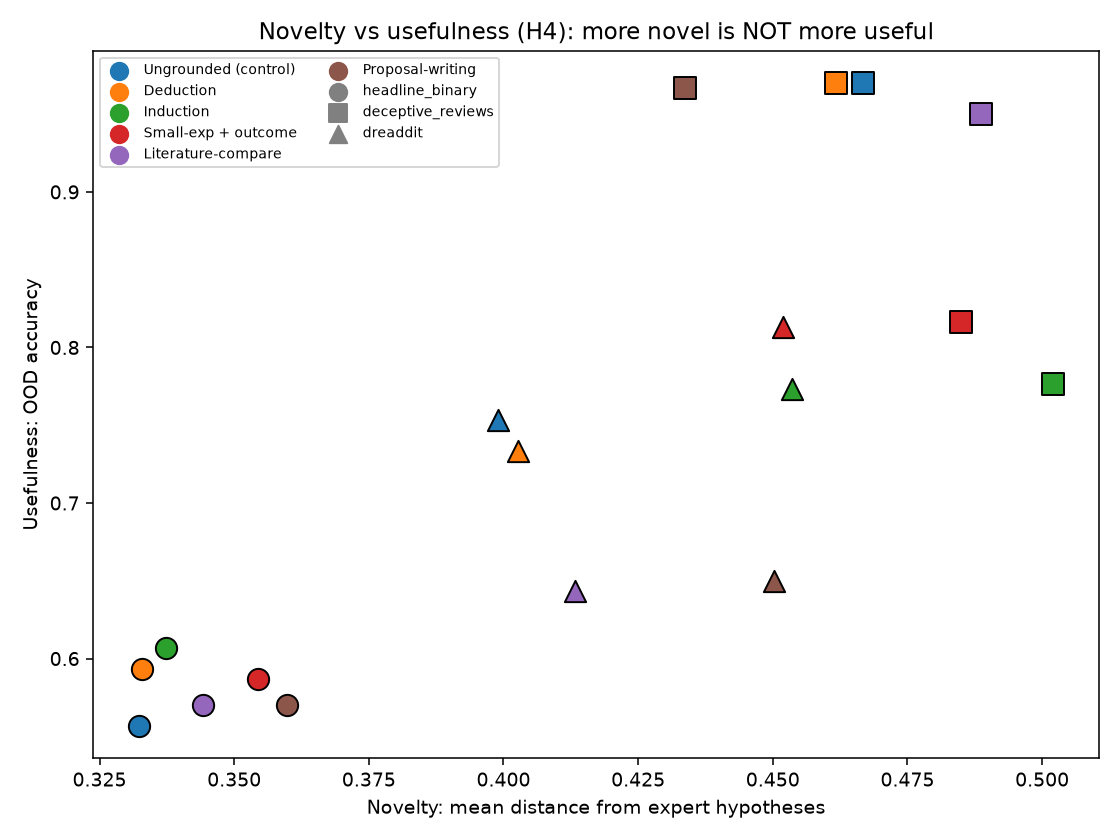
\includegraphics[width=\textwidth]{figures/fig3_novelty_vs_usefulness.png}
\caption{Novelty vs.\ usefulness}
\label{fig:novelty}
\end{subfigure}
\caption{\captiona{} \figleft{} Generation tokens per bank vs.\ \IND{} accuracy:
empirical grounding (C3) buys its gain at $\sim\!80\times$ the control's token cost,
while cheaper grounded regimes do not beat the control. \captionb{} \figright{} Bank
novelty (distance from expert hypotheses) vs.\ \OOD{} usefulness: the strong pooled
correlation is a task-difficulty confound that vanishes within task, so novelty does
not track usefulness.}
\label{fig:costnovelty}
\end{figure}

\section{Discussion}
\label{sec:discussion}

\para{Why ungrounded is so strong now.} The control's banks already recite the
\emph{right} expert-level features. For \dreaddit, \gptmini{} ungrounded produces
textbook stress markers---first-person pronouns, absolutist words, sleep disturbance,
inability to cope---without ever seeing data. A strong model's parametric prior is
itself a form of grounding, acquired in pretraining. This is the crux of our partly
negative result: the 2023-era finding ``grounding beats ungrounded prompting'' was
measured against much weaker baselines; with a 2025 model the ungrounded control is a
strong, often-transferable starting point, which shrinks grounding's headroom.

\para{Why empirical grounding is the exception.} \Cempirical{} (C3) is the only
regime that changes its ideas in response to evidence: it tests the bank, observes
concrete mistakes, and revises, producing richer rules (\eg ``intrusive thoughts /
trauma / self-blame with ongoing distress''). This closed loop is exactly the ``small
experiments + outcome imagination'' grounding the hypothesis names, and it is the one
mechanism that reliably lifts \IND{} accuracy ($d{=}1.09$). The catch is twofold: its
\IND{} gain does not transfer \OOD, and it is by far the most expensive regime
($\sim\!80\times$ tokens).

\para{Why proposal writing backfires.} Distilling a prose proposal into rules yields
rigid, symmetric ``if high $X$ $\rightarrow$ A / if low $X$ $\rightarrow$ B''
statements with the lowest diversity of any regime. The elaboration adds words, not
discriminative power, and the brittle thresholds misfire. This is a concrete instance
of LLM ideation that looks thorough while being measurably less useful---a warning
against equating structured elaboration with idea quality.

\para{The overfitting result.} On \deceptive, data grounding helped \IND{} but
\emph{hurt} \OOD, because the learned rules encode dataset-specific surface cues that
do not transfer, whereas the ungrounded prior captures general structure that does.
Prior work emphasizes data grounding's \OOD{} \emph{wins}; under one protocol with a
strong model we find it can \emph{trade} \OOD{} robustness for \IND{} fit. (Here
\deceptive's \OOD{} split is in fact easier than its \IND{} split for general priors,
which amplifies the effect; the within-split grounded-vs-ungrounded comparison still
holds.) The practical lesson is that ``ground in data'' should come with an
\OOD{} check, not an assumption of transfer.

\para{Verdict on the hypotheses.} The hypothesis ``grounding makes LLM ideas better''
is \emph{refuted as a blanket claim} but \emph{supported for one specific mechanism}.
H1 (grounding helps overall) is not supported. H2 (empirical grounding strongest) is
partially supported: empirical grounding leads \IND, but the full predicted ordering
does not hold. H3 (grounding helps most \OOD) is not supported---often the reverse.
H4 (novelty $\neq$ usefulness) is confirmed once the task-difficulty confound is
removed. The headline takeaway: ``ground your ideation'' is too coarse a prescription
for today's strong LLMs; \emph{grounding in empirical feedback} is the one mechanism
that reliably adds value, pure elaboration harms, and data grounding's benefit is
conditional.

\para{Limitations.} (1)~\emph{Tasks and construct.} We use three binary text-classification
tasks (one near chance), and operationalize ``idea quality'' as downstream label
accuracy. This captures grounded usefulness but not open-ended scientific
creativity; idea-level benchmarks were out of scope. (2)~\emph{Single model family.}
Generator and evaluator are both \gptmini. A stronger ungrounded baseline would
likely shrink grounding's value further, while a weaker model might restore the
classic grounding wins; cross-model replication is the key next step.
(3)~\emph{Power.} We have $9$ paired cells per comparison (and only $6$ points per
task for the within-task novelty analysis); effect \emph{directions} are clear, but
some non-significant results may be power-limited, and \headline{} contributes mostly
noise. (4)~\emph{One instantiation per regime.} Each grounding mechanism is one
reasonable design; stronger literature grounding (real retrieval over papers) or
longer empirical loops could change the standings. (5)~\emph{Evaluator ceiling.} A
single shared evaluator is fair across regimes but caps the measurable quality of any
hypothesis.

\para{Broader implications.} For practitioners, the message is to spend grounding
effort where it pays: a cheap ungrounded prompt of a capable model is a strong
default, empirical test-and-revise is worth its cost when in-distribution accuracy is
the goal and budget allows, and structured elaboration should be treated with
suspicion. For researchers, single-grounding comparisons against weak baselines can
overstate grounding's value; mechanism-level, single-protocol ablations with strong
controls give a more honest picture.

\section{Conclusion}
\label{sec:conclusion}

We presented the first single-protocol, head-to-head ablation of six LLM ideation
regimes---one ungrounded control and five grounding mechanisms---holding the model,
task suite, generation budget, and evaluation procedure fixed and scoring each by
objective downstream utility. Our answer to the motivating question is nuanced and
partly negative: under a fixed, objective protocol, \emph{grounding does not reliably
make a strong LLM's ideas better}. Pooled across mechanisms, grounded banks are
statistically indistinguishable from a strong ungrounded control.

\para{Key findings.} The mechanism is what matters. Grounding in empirical feedback
(test-and-revise) is the only regime that significantly improves in-distribution
usefulness ($+4.4$ points, $d{=}1.09$), but it costs $\sim\!80\times$ the tokens and
its gains do not transfer out-of-distribution. Pure elaboration (proposal writing)
significantly \emph{hurts} and collapses idea diversity. Data grounding can
\emph{overfit}, trading out-of-distribution robustness for in-distribution fit. And
novelty and diversity do not track usefulness within a task. Ungrounded prompting of
a capable model is a surprisingly hard baseline to beat.

\para{Future work.} Four directions follow directly. (1)~A cross-model sweep from
weaker to frontier generators, to map where grounding's value lives as the ungrounded
baseline strengthens. (2)~Regularized or \OOD-aware empirical grounding that keeps the
in-distribution gain without overfitting to surface cues. (3)~Idea-level domains
(\eg rediscovery benchmarks) to test whether these conclusions hold for open-ended
ideation rather than classification rules. (4)~Hybrid ``prior $+$ minimal empirical
check'' regimes that aim to capture most of empirical grounding's gain at a fraction
of its cost. We release all banks, per-item predictions, and statistics to support
these next steps.


\bibliography{references}

\end{document}
